\documentclass[tikz,border=10pt]{standalone}
\usepackage{tikzducks}
\begin{document}
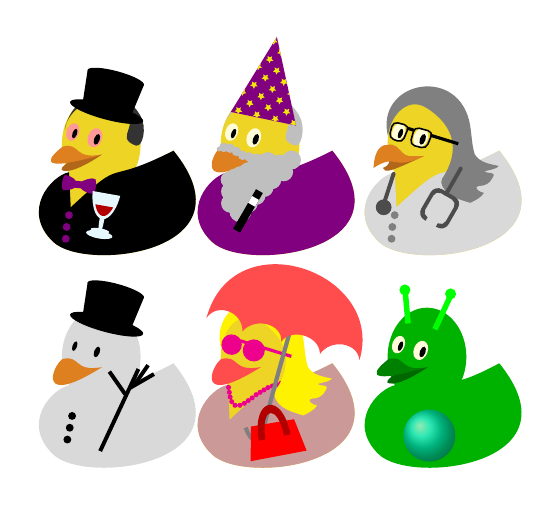
\begin{tikzpicture}
\node [matrix] {
  \duck[laughing, tophat, bowtie=violet, jacket=black,
    buttons=violet, recedinghair=black!80, 
    wine, eye=red!40] &
  \duck[magichat, recedinghair=lightgray,
      jacket=violet, beard=lightgray, magicwand] &
  \duck[parrot, stethoscope=black!70, jacket=gray!30,
      buttons=gray, squareglasses, longhair=gray] \\
  \duck[snowduck=lightgray!60] &
  \duck[umbrella=red!70, handbag=red, bill=red!70,
    jacket=pink!80!black, longhair=yellow,
    necklace=magenta, sunglasses=magenta] &
  \duck[alien, body=green!70!black, crystalball,
    bill=green!50!black, laughing] \\ };
\end{tikzpicture}
\end{document}
